\documentclass[a4paper]{article}

\usepackage[a4paper,top=2cm,bottom=2cm,left=3cm,right=3cm,marginparwidth=1.75cm]{geometry}
\usepackage[utf8]{inputenc}
\usepackage[T1]{fontenc}
\usepackage{textcomp}
\usepackage[ngerman]{babel}
\usepackage{amsmath, amssymb, nccmath}
\usepackage{accents}

\usepackage{multirow}

% figure support
\usepackage{import}
\usepackage{xifthen}
\pdfminorversion=7
\usepackage{pdfpages}
\usepackage{transparent}
\newcommand{\incfig}[1]{%
    \def\svgwidth{\columnwidth}
    \import{./figures/}{#1.pdf_tex}
}

\pdfsuppresswarningpagegroup=1

\title{Protokoll zur ersten Laborübung\\Messtechnik Labor 376.091}
\author{DINC Atilla (11917652)}

\begin{document}
\newcommand{\unit}[1]{\ensuremath{\, \mathrm{#1}}} % Einheiten in Math-Moder richtig formatieren
\normalsize
\maketitle
\tableofcontents

\begin{center}
	\begin{tabular}{|c| c| c| c| c|}
		\hline
		\multicolumn{5}{|c|}{\textbf{Geräteliste}}                                                                                        \\
		\hline

		Bezeichnung              & Gerätebeschreibung                                         & Messgrößen & Inventarnummer & Bemerkungen \\
		\hline
		MM0                      & Agilent Digitalmultimeter True RMS                                  & -          & U1232A         & -           \\
		MM1                      & Digitalmultimeter                                          & -          & #11            & -           \\
		MM2                      & Digitalmultimeter                                          & -          & #7             & -           \\
		\multirow{2}{*}{OZ1}     &
		\multirow{2}{*}{
			\begin{tabular}[c]
				Digitalspeicheroszilloskop DSO-x2002A \\
				MMSR
			\end{tabular}
		}                        &
		\multirow{2}{*}{-}     &
		\multirow{2}{*}{C0404-5} &
		\multirow{2}{*}{-}                                                                                                                \\
		                         &                                                            &            &                &             \\
		NG1                      & Netzgerät 2-Channel $\pm10\unit{mV}$                       & -   & CD0404-6       & -           \\
		FG1                      & Funktionsgenerator                                         & -    & SDG1025        & -           \\
		\hline
		\hline
		\multicolumn{5}{|c|}{\textbf{Zubehörliste}}                                                                                       \\
		\hline

		Bezeichnung              & Zubehörbeschreibung                                        & Messgrößen & Inventarnummer & Bemerkungen \\
		\hline
		K1                       & Tastkopf (10:1) 100\unit{MHz} 10\unit{M\Omega} 15\unit{pf} & -          & -              & rot         \\
		K2                       & Tastkopf (10:1) 150\unit{MHz} 10\unit{M\Omega} 15\unit{pf} & -          & -              & grau        \\
		K3                       & Tastkopf (10:1) 150\unit{MHz} 10\unit{M\Omega} 15\unit{pf} & -          & -              & rosa        \\
		\hline
	\end{tabular}
\end{center}
\newpage
% ~~~~~~~~~~~~~~~~~~~~~~~~~~~~ Start of the document ~~~~~~~~~~~~~~~~~~~~~~~~~~~~

\section{Einleitung}

\section{Messungen mit dem Digitalmultimeter}
\subsection{Spannungsmessung}
Zur Spannungsmessung wird der Spannungseingang des Multimeters parallel zur Messgröße
geschaltet, daher ist ein möglichst hoher Innenwiderstand $R_{i}$ erwünscht. Zur
Bestimmung dieses Innenwiderstands $R_{i}$ wird eine Serienschaltung mit einem 
relativ hochohmigen bekannten Widerstand aufgebaut und der Spannungsabfall am Multimeter
von diesem abgelesen.

\subsubsection{Mathematische Grundlagen}
\[ U_{V}=U_{q} \frac{R_{i}}{R_{1}+R_{i}} = U_{q} \frac{1}{1 + \frac{R_{1}}{R_{i}}}
        \implies R_{i}=\frac{R_{1}}{\frac{U_{q}}{U_{v}}-1} \]

\subsubsection{Messaufbau und Messdurchführung}
Die eingestellte Spannung des Netzgerätes FG1 wurde mit dem Multimeter MM2 
geprüft bevor sie mit der Schaltung belastet wurde. Der Serienwiderstand R1 wurde
mit dem Multimeter MM2 bestimmt.
Im Anschluss wurde die Schaltung wie in Abb. \ref{fig:RiVM} angeschlossen.
Die angezeigte Spannung am Multimeter MM1 wurde abgelesen und die Eingangsspannung
wurde erneut gemessen. Weder die Eingangsspannung, noch die Spannung am Multimeter
MM1 haben sich geändert. Somit wurde sichergestellt, dass sowohl Innenwiderstand
des Netzgerätes, alsauch jegliche Kontaktwiderstände in der Schaltung
vernachlässigbar klein für unsere Messungen waren.\newline
Der Kontrollprozess wurde bei Bedarf an anderen Schaltungen wiederholt.

\begin{figure}[h]
	\centering
	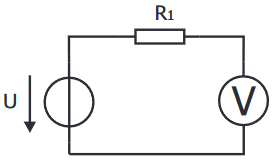
\includegraphics[width=0.8\textwidth]{schematics/1a_RiVM.png}
	\caption{Schaltung zur Bestimmung des Multimeter-Innenwiderstands}
	\label{fig:RiVM}
\end{figure}

\subsubsection{Messergebnisse}


\subsection{Strommessung}
Kurzbeschreibung hier \ref{fig:EinlussVM}
\begin{figure}[h]
	\centering
	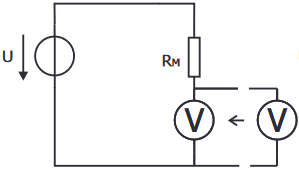
\includegraphics[width=0.8\textwidth]{schematics/1b_EinflussVM.png}
	\caption{Schaltung zur Messung des Einflusses durch die Messung}
	\label{fig:EinlussVM}
\end{figure}

\subsection{Widerstandsmessung}
\ref{fig:MB-Erweiterung}
\begin{figure}[h]
	\centering
	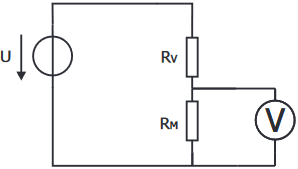
\includegraphics[width=0.8\textwidth]{schematics/1c_MessbereichserweiterungVM.png}
	\caption{Schaltung zur messbereichserweiterten Messung}
	\label{fig:MB-Erweiterung}
\end{figure}

\section{Messungen mit dem Oszilloskop}
\subsection{Tastkopf}
\subsection{AC-Spannungsmessung}
\subsection{RMS im Detail}
\subsection{Amplitudenauflösung}
\subsection{Dynamik}


\end{document}
